\documentclass[10pt,twocolumn]{article}
% Shared two-column preamble for the three research papers.
% Use with: \documentclass[10pt,twocolumn]{article}
% Then in main.tex: % Shared two-column preamble for the three research papers.
% Use with: \documentclass[10pt,twocolumn]{article}
% Then in main.tex: % Shared two-column preamble for the three research papers.
% Use with: \documentclass[10pt,twocolumn]{article}
% Then in main.tex: \input{../../shared/latex/twocolumn_preamble.tex}

\usepackage[margin=0.75in]{geometry}
\usepackage[utf8]{inputenc}
\usepackage[T1]{fontenc}
\usepackage{lmodern}
\usepackage{microtype}
\usepackage{amsmath,amssymb,amsthm}
\usepackage{graphicx}
\usepackage{booktabs}
\usepackage{caption}
\usepackage{subcaption}
\usepackage{hyperref}
\usepackage{url}
\usepackage{xcolor}
\usepackage{algorithm}
\usepackage{algorithmic}
\usepackage{multirow}
\usepackage{titlesec}
\usepackage{authblk}

\hypersetup{colorlinks=true,linkcolor=blue!50!black,citecolor=blue!50!black,urlcolor=blue!50!black}

\titleformat{\section}{\normalfont\large\bfseries}{\thesection}{0.6em}{}
\titleformat{\subsection}{\normalfont\bfseries}{\thesubsection}{0.5em}{}

\captionsetup{font=small,labelfont=bf,skip=4pt}
\setlength{\columnsep}{0.25in}
\setlength{\parskip}{2pt}

\newtheorem{theorem}{Theorem}
\newtheorem{proposition}[theorem]{Proposition}
\newtheorem{definition}[theorem]{Definition}


\usepackage[margin=0.75in]{geometry}
\usepackage[utf8]{inputenc}
\usepackage[T1]{fontenc}
\usepackage{lmodern}
\usepackage{microtype}
\usepackage{amsmath,amssymb,amsthm}
\usepackage{graphicx}
\usepackage{booktabs}
\usepackage{caption}
\usepackage{subcaption}
\usepackage{hyperref}
\usepackage{url}
\usepackage{xcolor}
\usepackage{algorithm}
\usepackage{algorithmic}
\usepackage{multirow}
\usepackage{titlesec}
\usepackage{authblk}

\hypersetup{colorlinks=true,linkcolor=blue!50!black,citecolor=blue!50!black,urlcolor=blue!50!black}

\titleformat{\section}{\normalfont\large\bfseries}{\thesection}{0.6em}{}
\titleformat{\subsection}{\normalfont\bfseries}{\thesubsection}{0.5em}{}

\captionsetup{font=small,labelfont=bf,skip=4pt}
\setlength{\columnsep}{0.25in}
\setlength{\parskip}{2pt}

\newtheorem{theorem}{Theorem}
\newtheorem{proposition}[theorem]{Proposition}
\newtheorem{definition}[theorem]{Definition}


\usepackage[margin=0.75in]{geometry}
\usepackage[utf8]{inputenc}
\usepackage[T1]{fontenc}
\usepackage{lmodern}
\usepackage{microtype}
\usepackage{amsmath,amssymb,amsthm}
\usepackage{graphicx}
\usepackage{booktabs}
\usepackage{caption}
\usepackage{subcaption}
\usepackage{hyperref}
\usepackage{url}
\usepackage{xcolor}
\usepackage{algorithm}
\usepackage{algorithmic}
\usepackage{multirow}
\usepackage{titlesec}
\usepackage{authblk}

\hypersetup{colorlinks=true,linkcolor=blue!50!black,citecolor=blue!50!black,urlcolor=blue!50!black}

\titleformat{\section}{\normalfont\large\bfseries}{\thesection}{0.6em}{}
\titleformat{\subsection}{\normalfont\bfseries}{\thesubsection}{0.5em}{}

\captionsetup{font=small,labelfont=bf,skip=4pt}
\setlength{\columnsep}{0.25in}
\setlength{\parskip}{2pt}

\newtheorem{theorem}{Theorem}
\newtheorem{proposition}[theorem]{Proposition}
\newtheorem{definition}[theorem]{Definition}

\newcommand{\OneOverE}{0.368}
\newcommand{\SecNhi}{1000}
\newcommand{\SecXstarHi}{0.368}
\newcommand{\SecPstarHi}{0.368}
\newcommand{\SecNlo}{10}
\newcommand{\SecXstarLo}{0.300}
\newcommand{\SecPstarLo}{0.399}
\newcommand{\ParkPhi}{0.90}
\newcommand{\ParkNaiveRegretHi}{1602.0}
\newcommand{\ParkPlo}{0.30}
\newcommand{\ParkNaiveRegretLo}{0.0}
\newcommand{\AgentSecN}{100}
\newcommand{\AgentQx}{0.390}
\newcommand{\AgentQregret}{1.4}
\newcommand{\AgentRex}{0.401}
\newcommand{\AgentReRegret}{17.6}
\newcommand{\ParkQregretHi}{0.0}
\newcommand{\ParkQregretLo}{16.9}
\newcommand{\CostMax}{0.0050}
\newcommand{\CostMaxXstar}{0.130}


\title{When Should You Stop Looking? The 37\% Rule, the Parking Problem,
and What Model-Free Agents Rediscover}
\author[1]{Luis Benvenuto}
\affil[1]{Independent Research}
\date{\today}

\begin{document}
\twocolumn[
\maketitle
\begin{@twocolumnfalse}
\begin{abstract}
\noindent The ``37\% rule'' states that when choosing sequentially from $n$
options you should reject the first $1/e$ of them and then take the next
record. We revisit this folklore result, place it inside a common
Markov-decision-process (MDP) skeleton alongside the parking problem of
MacQueen and Miller~(1960), and ask an empirical question: do model-free
reinforcement-learning agents, told nothing about the theory, rediscover the
optimal stopping thresholds from reward alone? Exact backward induction gives
computable ground truth. Tabular $Q$-learning recovers the secretary optimum
to within $\AgentQregret\%$ regret at $n=\AgentSecN$ and matches the parking
optimum exactly at high occupancy. In contrast, transplanting the $37\%$ rule
onto the parking problem is catastrophic --- its regret reaches
$\ParkNaiveRegretHi\%$ when free spots are common --- and a per-observation
search cost pulls the optimal cutoff from $\OneOverE$ down to
$\CostMaxXstar$. The $37\%$ rule is thus a fragile special case, not a
universal law of search; agents that learn from experience track the true,
problem-dependent threshold instead.
\end{abstract}
\vspace{1em}
\end{@twocolumnfalse}
]

\section{Introduction}
You are looking for a parking spot, driving toward your destination. Each spot
you pass is either free or taken, and once you drive past a free one you cannot
return. Stop too early and you walk a long way; hold out for the perfect spot
and you may overshoot and find nothing. When should you take what you have?

The popular answer invokes the \emph{secretary problem}: examine and reject the
first $37\%$ of the options, then take the next one that beats everything seen
so far. The cutoff $1/e\approx\OneOverE$ is genuinely optimal --- but only for
the exact problem the secretary story describes: a fixed, known number of
candidates, no recall, no cost to looking, and a payoff that rewards \emph{only}
selecting the single best. The parking problem violates several of these
assumptions, and the $37\%$ answer is simply wrong for it.

\paragraph{Question.} Two questions organise this paper. (i) How fragile is the
$37\%$ rule --- how far does the optimal stopping threshold move as we relax the
secretary assumptions toward the parking problem and toward costly search?
(ii) If an agent is given only the reward signal and no theory, does it
\emph{rediscover} the correct threshold from experience?

\paragraph{Approach.} We cast the classic secretary problem, the parking
problem, and two variants (a per-observation cost; cardinal ``full
information'') inside one MDP skeleton: observe, then \texttt{stop} or
\texttt{continue}. For the secretary problem the optimal policy has a
closed form; for the parking problem we obtain exact ground truth by backward
induction. Against these references we run tabular $Q$-learning and a
one-parameter policy-gradient (REINFORCE) learner.

\paragraph{Findings.} (i) The $37\%$ rule emerges cleanly only in the classic
rank-only, cost-free limit: at $n=\SecNhi$ the optimum sits at
$x^*=\SecXstarHi$ with success $\SecPstarHi$, but for $n=\SecNlo$ it is already
$\SecXstarLo$. (ii) Transplanted onto parking, the $37\%$ rule is disastrous:
regret up to $\ParkNaiveRegretHi\%$ at occupancy $p=\ParkPhi$. (iii) A search
cost of $\CostMax$ per look pulls the optimal secretary cutoff down to
$\CostMaxXstar$. (iv) $Q$-learning recovers the secretary optimum
($\AgentQregret\%$ regret at $n=\AgentSecN$) and the parking optimum (exact at
$p=\ParkPhi$) from reward alone; the one-parameter policy-gradient agent finds
the right regime but with higher variance.

\paragraph{Contributions.} A unified MDP treatment of the stopping family with
exact-DP ground truth; a quantification of how badly the $37\%$ rule fails off
its home turf; and an empirical study of what model-free agents recover.

\section{Related Work}
\paragraph{The secretary problem.} The best-choice problem and its $1/e$ law
were popularised in the 1960s; Ferguson~\cite{ferguson1989solved} traces its
tangled history and Freeman~\cite{freeman1983secretary} surveys the many
variants. Gilbert and Mosteller~\cite{gilbert1966recognizing} solved the
\emph{full-information} version, in which cardinal values (not just ranks) are
observed and the optimal win probability rises to $\approx 0.580$.

\paragraph{The parking problem.} MacQueen and Miller~\cite{macqueen1960optimal}
introduced the ``optimal persistence'' or parking formulation, where the payoff
depends on how far one stops from a goal rather than on picking a unique best.
It is the canonical example in which the $37\%$ intuition breaks down, because
the optimal rule is a distance threshold that depends on how often spots are
free.

\paragraph{Optimal stopping and RL.} Optimal stopping is a classical topic in
dynamic programming~\cite{chow1971great}; more recently it has been attacked
with reinforcement learning and neural function approximation, e.g.\ for
option pricing~\cite{becker2019deep}. Our aim is narrower and pedagogical:
using problems small enough to solve exactly, we ask what \emph{tabular},
assumption-free agents recover, and use the closed forms as ground truth rather
than as training signal.

\section{Problems and Optimal Policies}
All four problems share one skeleton: observe items in sequence; at each item
choose \texttt{stop} (commit, ending the episode) or \texttt{continue}. They
differ in what is observed and how the terminal reward is scored.

\subsection{Classic secretary (rank-only)}
$n$ candidates arrive in uniform random order; only relative ranks are visible;
the reward is $1$ iff the candidate committed to is the global best. The
optimal policy rejects the first $r$ candidates and then takes the first
\emph{record} (best-so-far). Its success probability is
\begin{equation}
P(r,n) = \frac{r}{n}\sum_{i=r+1}^{n}\frac{1}{i-1},
\label{eq:sec}
\end{equation}
and as $n\to\infty$ with $x=r/n$ this tends to $P(x)=-x\ln x$, maximised at
$x^\star=1/e$ with $P^\star=1/e$. We also score \emph{arbitrary} (possibly
non-threshold) policies exactly: a per-position take-mask $S$ wins with
probability $\sum_{i\in S}\tfrac1n\prod_{j<i,\,j\in S}\tfrac{j-1}{j}$, using the
independence of record events (Eq.~\ref{eq:sec} is the threshold special case).

\subsection{Parking problem}
Driving toward a destination, we pass spots at known distances
$c_1,\dots,c_T$ (we use $[k,\dots,1,0,1,\dots,k]$). Each spot is
\emph{free} independently with probability $p$. At a free spot we park (pay its
distance, stop) or skip; running off the end pays a penalty $F$. The expected
remaining cost obeys the backward recursion
\begin{equation}
V_t = p\,\min(c_t, V_{t+1}) + (1-p)\,V_{t+1},\qquad V_{T}=F,
\label{eq:park}
\end{equation}
so the optimal action at a free spot is to park iff $c_t \le V_{t+1}$. The
threshold $V_{t+1}$ is \emph{per-step}, not a single distance: near the end of
the street one accepts almost anything rather than fail. Equation~\ref{eq:park}
is exact and serves as ground truth for the agents.

\subsection{Variants}
\textbf{Costly search.} Each inspected candidate costs $c$; the payoff is
$P(\text{win}) - c\,\mathbb{E}[\#\text{inspected}]$. As $c$ grows the optimal
cutoff shrinks below $1/e$. \textbf{Full information.} Cardinal values are
observed; the optimal win probability rises toward $\approx0.580$
\cite{gilbert1966recognizing}, showing that the $37\%$ ceiling is an artefact
of discarding magnitude information.

\subsection{Agents}
Neither agent is given the closed forms. \emph{Tabular $Q$-learning} operates on
the discrete decision states (record position for secretary; street step for
parking) with two actions, an $\epsilon$-greedy behaviour policy, and linearly
annealed exploration and learning rate; we score its greedy policy exactly via
the formulas above. \emph{REINFORCE} learns a single threshold parameter passed
through a sigmoid, so the learned scalar \emph{is} the cutoff --- a natural fit
for the stationary secretary rule, but deliberately mis-specified for the
non-stationary parking optimum, which we use to illustrate that the policy
class, not just the learner, matters.

\section{Experimental Setup}
Everything is synthetic and config-driven; no external data or pretrained
models are used. The local configuration sweeps pool sizes
$n\in\{10,100,1000\}$ (agents trained on $\{10,50,100\}$, where the tabular
state space stays dense), parking occupancies $p\in\{0.3,0.5,0.7,0.9\}$ on a
street of half-length $k=8$ with failure penalty $F=20$, and observation costs
$c\in\{0,\dots,\CostMax\}$ at $n=100$. Monte-Carlo estimates use
$5\times10^4$ episodes per point; agents train for up to $8\times10^4$
episodes per cell over five seeds, and we report means with bootstrap $95\%$
confidence intervals. The \texttt{gpu\_full.yaml} configuration widens every
sweep and raises the episode and seed counts; no code changes are required.

Reproduce with \texttt{make all}: \texttt{run\_montecarlo} writes the
closed-form and simulated curves, \texttt{run\_agents} trains and scores the
learners, and \texttt{plot\_stopping} regenerates every figure together with
the numeric macros used in this text.

\section{Results}
\subsection{The 37\% rule and its finite-$n$ reality}
Figure~\ref{fig:seccurve} shows the success probability against the skip
fraction $x=r/n$ for $n=\SecNhi$: the Monte-Carlo estimates lie on the
closed-form curve $-x\ln x$, which peaks at $x=1/e$. But the clean $1/e$ answer
is asymptotic. Figure~\ref{fig:finiten} tracks the optimum as $n$ grows: at
$n=\SecNlo$ the best cutoff is $x^*=\SecXstarLo$ with success $\SecPstarLo$
(higher than $1/e$, since fewer candidates make the best easier to catch),
converging to $x^*=\SecXstarHi$, $P^*=\SecPstarHi$ only by $n=\SecNhi$. The
``$37\%$'' is a large-$n$ limit, not a rule for small menus.

\begin{figure}[t]
\centering
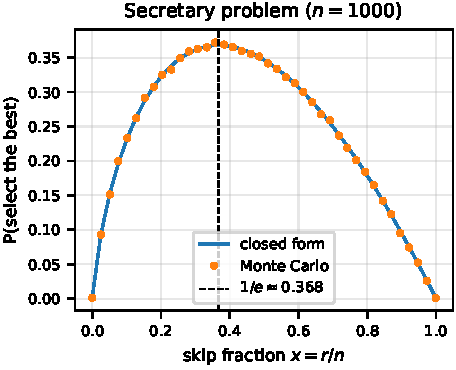
\includegraphics[width=\columnwidth]{figures/secretary_curve.pdf}
\caption{Secretary problem: Monte-Carlo success (points) matches the closed
form $-x\ln x$ (line); the optimum is at $x=1/e$.}
\label{fig:seccurve}
\end{figure}

\begin{figure}[t]
\centering
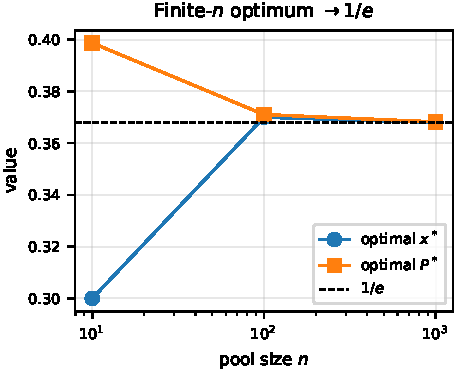
\includegraphics[width=\columnwidth]{figures/secretary_finite_n.pdf}
\caption{The optimal skip fraction $x^*$ and success $P^*$ approach $1/e$ only
as $n\to\infty$.}
\label{fig:finiten}
\end{figure}

\subsection{The 37\% rule fails on the parking problem}
Figure~\ref{fig:park} is the central result. The exact-DP optimum spends far
less than the naive rule that blindly skips the first $37\%$ of spots and then
takes the first free one. The gap widens sharply with occupancy: at
$p=\ParkPlo$ the naive rule is essentially optimal ($\ParkNaiveRegretLo\%$
regret), but at $p=\ParkPhi$ its regret explodes to $\ParkNaiveRegretHi\%$,
because when spots are usually free the right move is to hold out for the
destination itself, not to grab the first free spot after an arbitrary cutoff.

\begin{figure}[t]
\centering
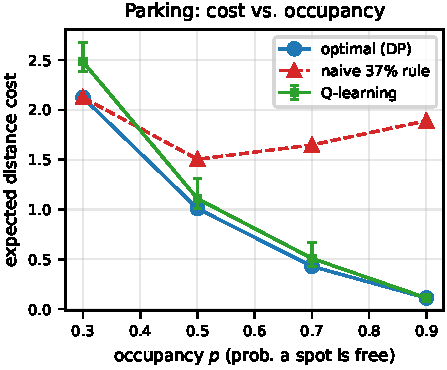
\includegraphics[width=\columnwidth]{figures/parking_cost.pdf}
\caption{Parking: expected walking cost vs.\ occupancy $p$. The learned
$Q$-agent tracks the DP optimum; the transplanted $37\%$ rule does not.}
\label{fig:park}
\end{figure}

\subsection{Search cost pulls the cutoff below 37\%}
When looking is costly, patience is penalised. Figure~\ref{fig:cost} shows the
optimal secretary cutoff falling monotonically from $1/e$ at $c=0$ to
$\CostMaxXstar$ at $c=\CostMax$: with an inspection cost, one should commit
earlier than the $37\%$ folklore suggests.

\begin{figure}[t]
\centering
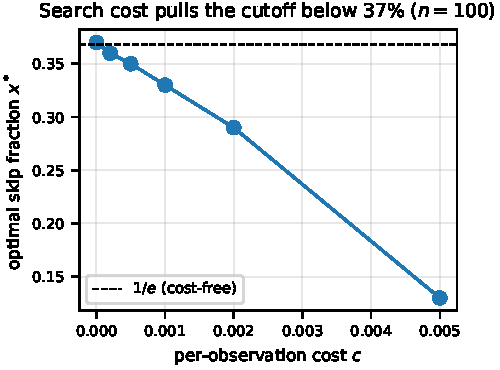
\includegraphics[width=\columnwidth]{figures/secretary_cost.pdf}
\caption{A per-observation cost pulls the optimal skip fraction below $1/e$.}
\label{fig:cost}
\end{figure}

\subsection{Agents rediscover the thresholds}
Given only rewards, tabular $Q$-learning recovers the secretary policy:
Figure~\ref{fig:agents} shows its learned cutoff concentrating near $1/e$, and
the greedy policy's exact success is within $\AgentQregret\%$ of optimal at
$n=\AgentSecN$. On parking --- the correct, per-step policy class --- it matches
the DP optimum exactly at $p=\ParkPhi$ and stays within $\ParkQregretLo\%$ in
the sparse-occupancy regime, where the acceptance boundary is hardest to pin
down from limited data. The one-parameter REINFORCE learner finds the right
secretary regime but with markedly higher variance ($\AgentReRegret\%$ regret),
and by construction cannot represent the non-stationary parking optimum ---
evidence that recovering the rule requires a policy class rich enough to hold
it.

\begin{figure}[t]
\centering
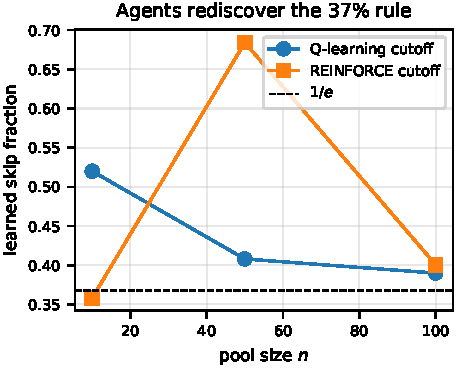
\includegraphics[width=\columnwidth]{figures/agents_secretary.pdf}
\caption{Learned skip fractions vs.\ pool size. $Q$-learning concentrates near
$1/e$; the policy-gradient cutoff is noisier.}
\label{fig:agents}
\end{figure}

\section{Discussion}
\paragraph{When does the 37\% rule actually apply?} Our sweeps make the
conditions concrete. The $1/e$ cutoff is close to optimal only when four things
hold at once: the number of options is fixed and reasonably large; you observe
ranks but care only about getting the single best; looking is free; and there is
no recall. Loosen any one and the threshold moves --- toward $0$ under search
cost, and toward the destination (hold out longer) as good options become
common in the parking problem. Treating $37\%$ as a universal heuristic for
apartments, dates, or parking spots is therefore usually wrong; the quantity
that transfers is the \emph{method} (compute the continuation value and stop
when the current option beats it), not the number.

\paragraph{What the agents tell us.} The value-based agent recovers the optimal
policy because its tabular representation can express the true, state-dependent
threshold, and because exact scoring lets us read off regret rather than a
noisy return. The policy-gradient agent's difficulty is instructive: a single
learned cutoff is the right hypothesis class for the stationary secretary rule
but cannot express the parking optimum at all. ``Learning the rule from
experience'' thus decomposes into two requirements --- enough data to estimate
the continuation values, and a policy class rich enough to hold the answer.

\paragraph{Limitations.} The problems are deliberately small so that exact
ground truth exists; we do not claim these particular learners scale to
high-dimensional stopping tasks. The parking model assumes independent
occupancy and a known street; correlated availability and unknown length are
natural next steps. The residual $Q$-learning regret in the sparse-occupancy
regime reflects finite-sample estimation of the acceptance boundary, not a
failure of the method, and shrinks under the larger-budget configuration.

\section{Conclusion}
The $37\%$ rule is a beautiful but narrow result: exact for the classic
secretary problem in the large-$n$, rank-only, cost-free limit, and badly wrong
once any of those assumptions slips. Placing the secretary and parking problems
in a common MDP with exact ground truth, we quantified the failure --- naive
regret up to $\ParkNaiveRegretHi\%$ on parking, and a cutoff dragged from
$\OneOverE$ to $\CostMaxXstar$ by a modest search cost --- and showed that a
tabular $Q$-learning agent, given only rewards, recovers the correct
problem-specific threshold where a one-parameter policy-gradient learner cannot.
The lesson for ``when to stop looking'' is not a magic percentage but a
procedure: estimate the value of continuing, and stop the moment your current
option beats it.


\bibliographystyle{plain}
\bibliography{references}

\end{document}
